\chapter{均匀空间的几何}

\lectureoverview{平坦性是对观测到的宇宙的极好近似，但它不是一条原理。如果我们保留均匀性和各向同性，同时允许存在曲率，那么会出现三种单连通的空间几何：欧几里得空间、球面空间和双曲空间。它们的度规可以由同心球壳随距离增长的方式构建，而它们的曲率可以通过角大小和天体计数来检验。当平坦空间的拓扑为环面时，它也可以是有限的。最后，将依赖于时间的尺度因子附加到这些均匀空间中的任何一个上，就给出了宇宙学时空度规和哈勃定律；该尺度因子的动力学必须来自广义相对论。}

\section{平坦性是一种观测结果，而非一条原理}

到目前为止，我们一直把空间当作平坦的，并且几乎未提及时空几何。观测使平坦空间成为一个非常好的近似，但这并没有把平坦性提升为一条定律。测量真正告诉我们的是，任何曲率半径都必须远大于我们已经勘测过的区域。空间可能是严格平坦的、正曲率的或负曲率的。在远超可观测区域的尺度上，我们尚不知道哪一种描述是正确的。

因此，我们放松一个假设，同时保留另一个假设。我们不再假设平坦性，但将继续假设空间是均匀且各向同性的。这是一个工作假设，而不是一条信条。为了了解它的推论，我们先假设它并进行计算；之后我们可以放弃它，并追问一个非均匀宇宙会有怎样不同的表现。

均匀性意味着每一点都具有相同的几何特征。一位观测者移动到别处并重复局部几何实验，会得到相同的结果。各向同性意味着没有哪个方向是特殊的。这些条件排除了人们最先画出的几乎所有曲面。抛物面在其顶点附近比远离顶点处弯曲得更剧烈。一个长椭球在其两极和腰部有所不同。一个带凸起的球面，或者把山脉和山谷分辨出来的地球表面，是弯曲的但不均匀。宇宙学的问题更狭窄：
\begin{quote}
哪些空间可以是弯曲的，同时从每一点、每个方向看过去在几何上仍然相同？
\end{quote}

暂时忽略整体拓扑识别，有三种常曲率答案：平坦空间、正曲率的球面空间和负曲率的双曲空间。关于整体拓扑识别的限定很重要；稍后我们将构造一个平坦的有限环面，并修正那种认为这三种已穷尽一切可能性的过度简化说法。

\section{度规与观测者的坐标}

我们首先只讨论空间，而不是时空。它的几何被编码在一个度规中：一条给出相邻点之间距离平方\(ds^2\)的规则。一旦这条局部规则处处已知，长度、角度、面积、体积、测地线和曲率都可以由它恢复出来。

对于欧几里得平面和欧几里得三维空间，笛卡儿坐标给出
\begin{equation}
ds_2^2=dx^2+dy^2,
\qquad
ds_3^2=dx^2+dy^2+dz^2.
\label{eq:c03-cartesian-flat}
\end{equation}
加上第三维只是添加了正交项\(dz^2\)，但要点并不在于这个公式的简单性。而在于方程~\eqref{eq:c03-cartesian-flat}完全指定了局部几何。

\begin{figure}[htbp]
\centering
\includegraphics[width=0.74\textwidth]{lecture_03_figure_02.png}
\caption{黑板上写出的平坦三维空间的笛卡儿度规。}
\label{fig:c03-cartesian-board}
\lectureframe{00:05:13.138}
\end{figure}

笛卡儿坐标掩盖了天文学家遭遇宇宙的方式。我们占据一个点，按方向向外看，并按角度和距离对所看到的东西进行分类。在一个二维宇宙中，视野实际上会是我们周围的一个方向圆。因此，极坐标不仅仅优雅；它们揭示了宇宙学所使用的角度几何。

设\(r\)为径向距离，\(\theta\)为方向。同一个欧几里得平面现在具有度规
\begin{equation}
ds^2 = dr^2 + r^2 d\theta^2.
\label{eq:c03-polar-flat}
\end{equation}
对于一个固定的小角度\(d\theta\)，横向间隔为\(r\,d\theta\)。它随着我们向外移动而线性增长，因此它对度规的平方贡献为\(r^2d\theta^2\)。

角度项本身就是一维空间的度规。圆是一个一维球面，记作\(S^1\)，而单位圆的度规按惯例写作
\begin{equation}
d\Omega_1^2 = d\theta^2,
\qquad\text{so that}\qquad
ds^2 = dr^2 + r^2 d\Omega_1^2.
\label{eq:c03-omega-one}
\end{equation}
黑板上写的是\(d\Omega^2\)，下标无法辨认；口头定义确定了所指的对象为\(d\Omega_1^2\)。

\begin{figure}[htbp]
\centering
\includegraphics[width=0.74\textwidth]{lecture_03_figure_03.png}
\caption{平坦空间的极坐标草图与度规。黑板上显示\(d\Omega^2\)；讲解说明它是单位圆度规\(d\Omega_1^2=d\theta^2\)。}
\label{fig:c03-polar-board}
\lectureframe{00:08:37.254}
\end{figure}

\begin{figure}[htbp]
\centering
\begin{tikzpicture}[scale=1.2]
\draw[->] (-1.2,0)--(1.8,0);
\draw[->] (0,-1.2)--(0,1.8);
\draw[thick] (0,0)--(1.3,1.1);
\draw (0.7,0.7) node[above] {$r$};
\draw (0.58,0) arc (0:40:0.58);
\draw (0.8,0.22) node {$\theta$};
\end{tikzpicture}
\caption{方程~\eqref{eq:c03-omega-one}中所用、以观测者为中心的极坐标的清晰重构图。}
\label{fig:c03-polar-redraw}
\end{figure}

\begin{classroomqa}
\audiencequestion{\(d\theta^2\)真的测量沿圆周的距离吗？}
\lecturerresponse{是的。在单位圆上，弧长等于以弧度计的角度，因此相隔\(d\theta\)的相邻点具有的固有间隔平方为\(d\theta^2\)。该圆的周长为\(2\pi\)，将\(ds=d\theta\)沿圆周积分一周恰好给出\(2\pi\)。乘以\(r^2\)将单位圆放大为平面中半径为\(r\)的壳层。\lecturetimestamp{00:09:11--00:09:26}}
\end{classroomqa}

\emph{固有}一词至关重要。若将单位圆嵌入欧几里得平面，我们可以用下式描述它：
\begin{equation}
x^2 + y^2 = 1.
\end{equation}
该方程描述的是圆如何位于一个更大的空间中。对于只能测量沿圆周距离的居民而言，并不需要它。我们可以把一根柔性光纤弯成一个不对称的闭合回路而不拉伸它。它在平面中的外观会改变，但其固有周长和度规不会改变。\(\theta\)的等增量仍将标记光纤上相等的距离。因此，几何必须与嵌入所赋予的偶然形状区分开来。

\begin{figure}[htbp]
\centering
\includegraphics[width=0.64\textwidth]{lecture_03_figure_04.png}
\caption{板书将圆形的单位圆与一个变形的闭合回路进行比较。如果回路被弯曲而不被拉伸，则二者具有相同的固有的一维度规。}
\label{fig:c03-intrinsic-board}
\lectureframe{00:10:34.205}
\end{figure}

\begin{figure}[htbp]
\centering
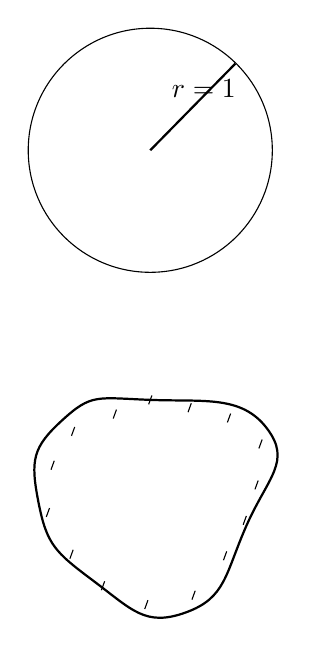
\begin{tikzpicture}[scale=1.0]
\draw (0,0) circle (1.55);
\draw[thick] (0,0)--(1.08,1.1);
\draw (0.68,0.78) node {$r=1$};

\begin{scope}[yshift=-4.35cm]
\draw[thick]
plot[smooth cycle, tension=0.95] coordinates
{(0,1.18) (1.48,0.82) (1.22,-0.42) (0.45,-1.52) (-0.72,-1.12) (-1.42,-0.12) (-1.12,0.92)};
\foreach \p in {(0,1.18),(0.5,1.08),(1.0,0.95),(1.4,0.62),(1.35,0.1),(1.2,-0.35),(0.95,-0.8),(0.55,-1.3),(-0.05,-1.42),(-0.6,-1.18),(-1.0,-0.78),(-1.3,-0.25),(-1.24,0.35),(-0.98,0.78),(-0.45,1.0)}{
\draw[rotate around={70:\p}] \p ++(-0.06,0) -- ++(0.12,0);
}
\end{scope}
\end{tikzpicture}
\caption{固有距离在外在形变下保持不变：一维居民在任一种嵌入中都测得相同的周长。}
\label{fig:c03-intrinsic-redraw}
\end{figure}

现在可以把平坦空间理解为围绕观测者的一族嵌套圆。距离为\(r\)处的壳层是单位圆被\(r\)放大后的副本，而这正是因子\(r^2d\Omega_1^2\)所记录的内容。

\section{正曲率：闭合的壳层}

球面是弯曲的，但却是均匀的：在完美圆球上，没有任何一点在几何上与其他点相区别。我们可以不借助外部的三维图像来构造其度规。设想生活在单位\(2\)球面上的二维天文学家，并将他们坐标的原点置于自身所在位置。

他们周围测地距离\(r\)处的圆很小。随着\(r\)增大，这些圆变大，在绕球面一半处达到最大周长，然后收缩，直到在对跖点处坍缩。这种增长和收缩随\emph{距离}发生，而不是随时间发生。在整个构造过程中，球面都是静态的。

这里\(r\)是沿单位球面的角距离，而不是距某个中心的欧几里得距离：
\[
0 \le r \le \pi.
\]
在\(r=0\)处是所选原点，在\(r=\pi/2\)处是绕行一半的大圆，在\(r=\pi\)处是对跖点。壳层的半径现在是\(\sin r\)，因此平坦因子\(r^2\)被替换为\(\sin^2r\)：
\begin{equation}
d\Omega_2^2 = dr^2 + \sin^2 r\, d\Omega_1^2
            = dr^2 + \sin^2 r\, d\theta^2.
\label{eq:c03-two-sphere}
\end{equation}
端点和中点的行为完全符合要求：
\begin{equation}
\sin 0=0,
\qquad
\sin\frac{\pi}{2}=1,
\qquad
\sin\pi=0.
\end{equation}
因此，这些壳层从零大小开始，达到最大大小，然后再次闭合。

\begin{figure}[htbp]
\centering
\includegraphics[width=0.82\textwidth]{lecture_03_figure_05.png}
\caption{从平坦空间中的嵌套圆到球面上的壳层的过渡。下方公式在画面中部分被遮挡；其口头推导给出了方程~\eqref{eq:c03-two-sphere}中的替换\(r^2\mapsto\sin^2r\)。}
\label{fig:c03-spherical-board}
\lectureframe{00:16:11.701}
\end{figure}

\begin{figure}[htbp]
\centering
\resizebox{\linewidth}{!}{%
\begin{tikzpicture}[scale=0.92]
\begin{scope}[xshift=-4.15cm]
\draw[->] (-1.7,0)--(1.9,0);
\draw[->] (0,-1.7)--(0,1.9);
\draw (0,0) circle (0.45);
\draw (0,0) circle (0.9);
\draw (0,0) circle (1.35);
\draw[thick] (0,0)--(1.45,1.2);
\draw (0.56,0.18) arc (18:40:0.63);
\draw (0.94,0.44) node {$\theta$};
\end{scope}

\begin{scope}[xshift=4.15cm]
\draw (0,0) circle (2.0);
\fill (0,-2.0) circle (1.5pt);
\fill (2.0,0) circle (1.5pt);
\fill (0,2.0) circle (1.5pt);
\draw[thick] (0,-2.0) arc (-90:90:2.0);
\draw (0,-2.35) node {$r=0$};
\draw (2.75,0) node {$r=\pi/2$};
\draw (0,2.35) node {$r=\pi$};
\end{scope}
\end{tikzpicture}
}%
\caption{平坦壳层永远增长，而球面壳层增长到\(r=\pi/2\)处的最大值，并在\(r=\pi\)处闭合。}
\label{fig:c03-shells-flat-sphere}
\end{figure}

记号\(d\Omega_2^2\)表示单位\(2\)球面的度规，正如\(d\Omega_1^2\)表示其圆形壳层的度规。同样的递归构造在更高一维中也成立。在平坦三维空间中固定半径处，我们周围的壳层是一个\(2\)球面：
\begin{equation}
ds_{\text{flat},3}^2 = dr^2 + r^2 d\Omega_2^2.
\label{eq:c03-flat-three-polar}
\end{equation}
如果这些\(2\)球面壳层以因子\(\sin r\)增长然后闭合，则所得空间是一个单位\(3\)球面：
\begin{equation}
d\Omega_3^2 = dr^2 + \sin^2 r\, d\Omega_2^2.
\label{eq:c03-three-sphere}
\end{equation}
\(3\)球面难以想象，因为其熟悉的嵌入需要四个欧几里得维度。然而，度规是完备的，不需要图像。围绕任何选定的观测者都有嵌套的\(2\)球面；它们增长到最大，然后收缩到对跖点。

\begin{classroomqa}
\audiencequestion{观测者位于球面的中心吗？}
\lecturerresponse{观测者位于\emph{坐标壳层}的中心，而不是某个特殊的几何中心。原点是空间中的一个点，任何其他观测者都可以选择自己的点作为\(r=0\)，并得到相同的度规。均匀性恰恰是说，不存在任何被偏好的此类选择。\lecturetimestamp{00:19:21--00:20:27}}
\end{classroomqa}

仅为了可视化，单位圆和单位\(2\)球面可以嵌入欧几里得空间：
\begin{equation}
x^2+y^2=1,
\qquad
x^2+y^2+z^2=1.
\end{equation}
这些方程描述的是嵌入，而不是额外的物理。被限制在圆或球面上的蚂蚁可以确定内禀度规，而无需探测周围的欧几里得空间。同样，\(S^3\)并不是一个带有神秘边界的普通球。它是由方程~\eqref{eq:c03-three-sphere}所描述的完整三维空间。

\section{曲率如何改变我们所看到的}

只有当几何改变观测时，几何才成为物理。假设一个物体具有已知的横向直径\(d\)，其径向距离\(r\)已被独立推断出来，并且其角直径\(d\theta\)在天上被测量到。星系提供了一个粗略的直观例子；更精确的宇宙学使用经过校准的标准尺和标准烛光。距离信息可以从光谱红移、哈勃关系、光度以及不同类别天体之间的交叉校准中汇集起来。

在平坦空间中，在物体的横向宽度上保持\(r\)固定。方程~\eqref{eq:c03-polar-flat}给出
\begin{equation}
d^2 = r^2 d\theta^2.
\label{eq:c03-flat-angle-step}
\end{equation}
因此
\begin{equation}
d\theta = \frac{d}{r}.
\label{eq:c03-flat-angle}
\end{equation}
角大小与距离成反比下降。

在单位球面上，横向壳层大小是\(\sin r\)而不是\(r\)：
\begin{equation}
d^2 = \sin^2 r\, d\theta^2,
\qquad\text{hence}\qquad
d\theta = \frac{d}{\sin r}.
\label{eq:c03-spherical-angle}
\end{equation}
对于\(0<r<\pi\)，\(\sin r<r\)，因此同一物体在相同径向距离处看起来比在平坦空间中更大。它的角大小先减小，在赤道处达到最小值，然后随着壳层收缩而增大。在对跖点处的极限理想化中，所有方向汇聚在一起，图像散布到整个天空。

\begin{classroomqa}
\audiencequestion{这与从宇宙微波背景推断曲率所用的想法相同吗？}
\lecturerresponse{是的。早期等离子体通过其声学振荡提供了一个特征物理尺度。我们测量那把标准尺所张的角，并将其与每种几何所预言的角进行比较。这些物体不必真的是星系；本质的比较是将已知的横向尺度与其观测到的角大小相对照。\lecturetimestamp{00:37:37--00:38:12}}
\end{classroomqa}

壳层体积提供了第二个检验。在三维平坦空间中，壳层的面积正比于\(r^2\)；在单位\(3\)球面上，它正比于\(\sin^2r\)。因此，一个均匀的总体在球面壳层上先随距离变得更加众多，然后在赤道之后变得更少。正曲率相对于平坦空间预言了一个成对的信号：足够远的标准尺看起来太大，而足够远的壳层包含的物体太少。

\begin{figure}[htbp]
\centering
\resizebox{\linewidth}{!}{%
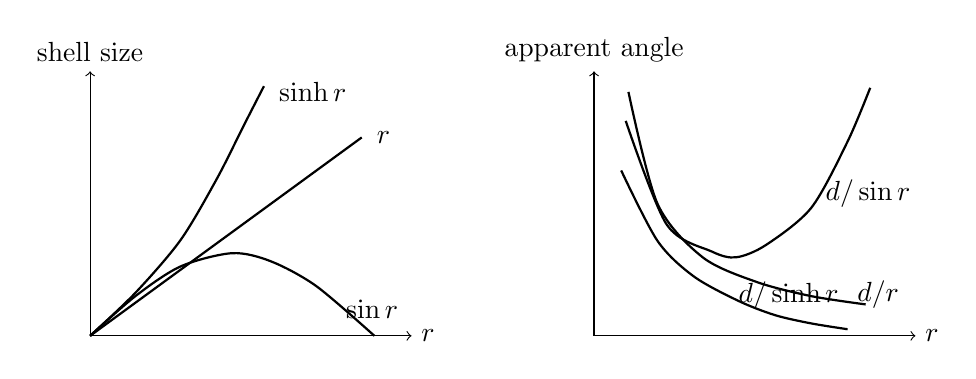
\begin{tikzpicture}[x=1.15cm,y=1.05cm]
\begin{scope}
\draw[->] (0,0)--(3.55,0) node[right] {$r$};
\draw[->] (0,0)--(0,3.2) node[above] {shell size};

\draw[thick] (0,0)--(3.0,2.4);
\draw (3.06,2.4) node[right] {$r$};

\draw[thick]
plot[smooth] coordinates {(0,0) (0.5,0.48) (1.0,0.84) (1.57,1.0) (2.0,0.9) (2.5,0.6) (3.14,0)};
\draw (2.72,0.55) node[below right] {$\sin r$};

\draw[thick]
plot[smooth] coordinates {(0,0) (0.5,0.52) (1.0,1.16) (1.4,1.9) (1.7,2.55) (1.92,3.02)};
\draw (1.98,2.95) node[right] {$\sinh r$};
\end{scope}

\begin{scope}[xshift=6.4cm]
\draw[->] (0,0)--(3.55,0) node[right] {$r$};
\draw[->] (0,0)--(0,3.2) node[above] {apparent angle};

\draw[thick]
plot[smooth] coordinates {(0.38,2.95) (0.7,1.6) (1.2,0.95) (1.8,0.65) (2.4,0.48) (3.0,0.38)};
\draw (2.8,0.5) node[right] {$d/r$};

\draw[thick]
plot[smooth] coordinates {(0.35,2.6) (0.8,1.35) (1.3,1.02) (1.57,0.95) (1.9,1.1) (2.4,1.55) (2.8,2.35) (3.05,3.0)};
\draw (2.45,1.72) node[right] {$d/\sin r$};

\draw[thick]
plot[smooth] coordinates {(0.3,2.0) (0.7,1.15) (1.1,0.72) (1.6,0.42) (2.0,0.25) (2.4,0.15) (2.8,0.08)};
\draw (2.15,0.2) node[above] {$d/\sinh r$};
\end{scope}
\end{tikzpicture}
}%
\caption{径向壳层因子及相应的角大小定律。正曲率使壳层闭合；负曲率使它指数增长。}
\label{fig:c03-shell-angular-laws}
\end{figure}

\begin{classroomqa}
\audiencequestion{当我们继续绕球面一周时，径向坐标会变成无穷大吗？}
\lecturerresponse{不会。在单位球面上，\(r\)是测地角距离，其范围仅为\(0\)到\(\pi\)。在\(r=\pi\)处，壳层已在对跖点坍缩。我们在这里考察的是一个固定的空间几何，而不是随时间跟随一个物体向外运动。稍后引入曲率半径会将所有物理距离乘以该半径，但不会改变这个无量纲的范围。\lecturetimestamp{00:39:30--00:40:35}}
\end{classroomqa}

\section{投影不是几何}

在转向负曲率之前，先看看一个忠实的几何能被一幅图扭曲到何种程度是有益的。把球面放在与其南极相切的平面上。从北极过球面上的每一点\(P\)画一条线，并延长到平面上的\(P'\)。这就是球极投影。北极本身被送到无穷远。南极附近的小区域被表示时几乎没有畸变，而北极附近相等的内禀区域在平面上变得极其巨大。

畸变属于地图，而不属于球面。源球面仍然是均匀的，尽管它的平面图像给等价区域赋予了截然不同的坐标大小。当把一个无限的双曲空间压缩到一个有限圆盘中时，将再次需要这种自律。

\begin{figure}[htbp]
\centering
\resizebox{\linewidth}{!}{%
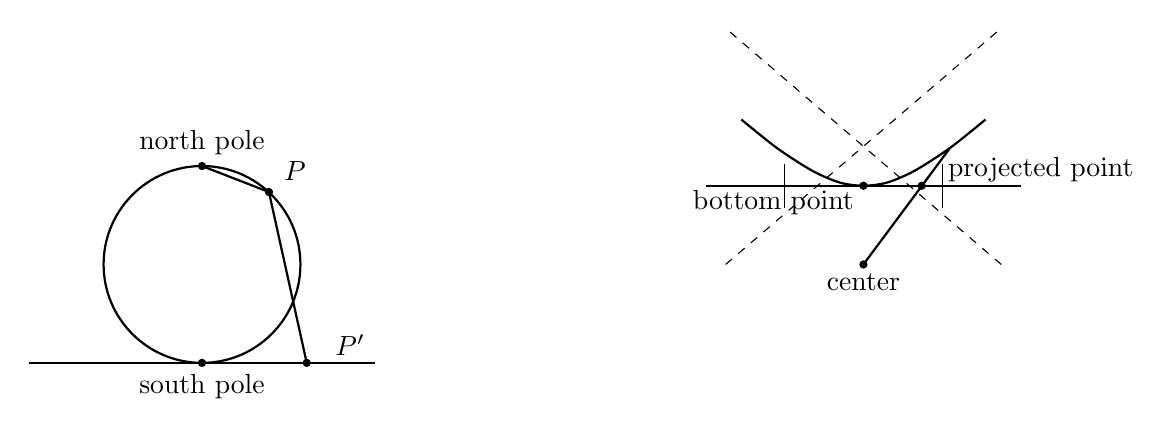
\begin{tikzpicture}[scale=1.0]
\begin{scope}[xshift=-4.2cm]
\draw[thick] (-2.2,-1.25)--(2.2,-1.25);
\draw[thick] (0,0) circle (1.25);
\fill (0,1.25) circle (1.5pt);
\fill (0,-1.25) circle (1.5pt);
\draw (0,1.55) node {north pole};
\draw (0,-1.55) node {south pole};

\fill (0.85,0.92) circle (1.5pt);
\draw (0.92,1.18) node[right] {$P$};
\draw[thick] (0,1.25)--(0.85,0.92)--(1.33,-1.25);
\fill (1.33,-1.25) circle (1.5pt);
\draw (1.57,-1.03) node[right] {$P'$};
\end{scope}

\begin{scope}[xshift=4.2cm]
\draw[thick] (-2.0,1)--(2.0,1);
\draw[dashed] (-1.75,0)--(1.75,3.0);
\draw[dashed] (1.75,0)--(-1.75,3.0);
\draw[thick]
plot[smooth] coordinates
{(-1.55,1.84) (-1.1,1.48) (-0.65,1.19) (-0.3,1.04) (0,1.0) (0.3,1.04) (0.65,1.19) (1.1,1.48) (1.55,1.84)};
\fill (0,0) circle (1.5pt);
\fill (0,1) circle (1.5pt);
\draw (0,-0.22) node {center};
\draw (0,0.78) node[left] {bottom point};
\draw[thick] (0,0)--(1.1,1.48);
\fill (0.74,1.0) circle (1.5pt);
\draw (0.95,1.2) node[right] {projected point};
\draw (-1,0.72) -- (-1,1.28);
\draw (1,0.72) -- (1,1.28);
\end{scope}
\end{tikzpicture}
}%
\caption{左：球极投影将球面的北极送到无穷远。右：双曲面可以投影到一个有限圆盘内，这里用一条截面区间表示。坐标畸变不会破坏内禀均匀性。}
\label{fig:c03-projections}
\end{figure}

\section{负曲率：超出平坦空间的球壳}

第三种单连通均匀几何将\(\sin r\)替换为双曲正弦。它在二维和三维中的单位度规为
\begin{equation}
dh_2^2 = dr^2 + \sinh^2 r\, d\Omega_1^2,
\label{eq:c03-hyperbolic-two}
\end{equation}
\begin{equation}
dh_3^2 = dr^2 + \sinh^2 r\, d\Omega_2^2.
\label{eq:c03-hyperbolic-three}
\end{equation}
坐标\(r\)现在的取值范围是
\begin{equation}
0\le r<\infty.
\end{equation}
在原点附近，\(\sinh r\approx r\)，因此该几何局部是欧几里得的。在远处，其球壳比欧几里得球壳增长得快得多，并且永远不会回转。

增长规律来自
\begin{equation}
\sin r = \frac{e^{ir}-e^{-ir}}{2i},
\qquad
\sinh r = \frac{e^r-e^{-r}}{2}.
\label{eq:c03-sin-sinh}
\end{equation}
在\(r\)很大时，\(\sinh r\sim e^r/2\)。因此，在二维中，周长随半径指数增长；在三维中，球壳面积按\(\sinh^2r\sim e^{2r}/4\)增长。均匀分布相应地在一个遥远球壳上包含同样多的物体。

对于一个横向大小为\(d\)的物体，
\begin{equation}
d^2 = \sinh^2 r\, d\theta^2,
\qquad\text{so}\qquad
d\theta = \frac{d}{\sinh r}.
\label{eq:c03-hyperbolic-angle}
\end{equation}
在\(r\)很大时，
\begin{equation}
d\theta \sim 2d\,e^{-r}.
\end{equation}
因此，负曲率给出的特征与正曲率相反：遥远的标准尺看起来太小，而遥远的球壳相对于平坦空间包含太多物体。

\begin{classroomqa}
\audiencequestion{径向范围如何区分球面和双曲空间？}
\lecturerresponse{在单位球面上，\(r\)止于对跖点，\(r=\pi\)。在双曲空间中，它无界地继续，\(0\le r<\infty\)。球壳因子揭示了同样的对比：\(\sin r\)回到零，而\(\sinh r\)永远增大。\lecturetimestamp{00:52:46--00:53:25}}
\end{classroomqa}

有一种嵌入使均匀性不那么神秘。引入环境坐标\(T,x,y\)，其中\(T\)只是一个嵌入坐标，而\emph{不是}宇宙学时间，并取上叶
\begin{equation}
T^2 - x^2 - y^2 = 1.
\label{eq:c03-hyperboloid}
\end{equation}
给环境空间配备洛伦兹号差度规
\begin{equation}
d\ell_{\mathrm{emb}}^2=-dT^2+dx^2+dy^2.
\label{eq:c03-ambient-minkowski}
\end{equation}
双曲面上诱导的度规是正定的。洛伦兹变换同时保持方程~\eqref{eq:c03-hyperboloid}和~\eqref{eq:c03-ambient-minkowski}，并且可以把上叶的任意点移到任意其他点。在这个意义上，改变双曲空间上的原点就像在辅助环境空间中倾斜时间轴。每个点在几何上都是等价的。

将双曲面投影到圆盘中，无穷远处的点会聚集在边界圆上。附近区域被画得几乎保真；更远的区域则被压缩得越来越强。这就是从天使与魔鬼的重复图形中熟悉的Poincar\'e圆盘表示。坐标变换可以把边缘附近一个看似很小的图形移到中心，在那里它变得很大，同时保持所有内禀长度和角度不变。在三维中，相应的模型是球而不是圆盘。\emph{Poincar\'e空间}、\emph{罗巴切夫斯基空间}和\emph{均匀负曲率空间}这些名称指的都是同一种局部几何。

\begin{classroomqa}
\audiencequestion{这个有限圆盘像彭罗斯图吗？}
\lecturerresponse{在有限图像内部表示无限区域这一有限意义上，它是相似的。然而在这里，圆盘只表示空间，而不是时空或因果无穷。尽管图中把它放在有限的坐标半径处，它的边界在内禀双曲度规中却位于无穷远处。\lecturetimestamp{01:02:55--01:03:05}}
\end{classroomqa}

\section{曲率半径}

到目前为止写出的度规描述的是单位几何。要给球面或双曲空间一个任意曲率半径，就把每个长度乘以一个常数。板书用\(a\)表示该常数；为了避免与后面使用的随时间变化的宇宙学尺度因子混淆，我们将把静态曲率半径称为\(R_c\)。由于度规测量的是长度的平方，
\begin{align}
ds_{\mathrm{sph}}^2
  &=R_c^2d\Omega_n^2
   =R_c^2\left(dr^2+\sin^2r\,d\Omega_{n-1}^2\right),\\
ds_{\mathrm{hyp}}^2
  &=R_c^2dh_n^2
   =R_c^2\left(dr^2+\sinh^2r\,d\Omega_{n-1}^2\right).
\label{eq:c03-scaled-curvature}
\end{align}
物理径向距离是\(R_cr\)。增大\(R_c\)会使空间曲率变小；恒定截面曲率的大小按\(1/R_c^2\)缩放。在\(R_c\to\infty\)的极限下，两个弯曲度规在每个固定的有限区域上都趋近欧几里得几何。

\begin{classroomqa}
\audiencequestion{如果球面变为两倍大，它会变得更弯曲还是更不弯曲？}
\lecturerresponse{更不弯曲。课堂上给出的第一个答案通过把篮球与地球作比较得到了纠正：较小的曲面在给定距离上弯曲得更快。将\(R_c\)加倍会使反半径曲率尺度减半，并使截面曲率\(1/R_c^2\)除以四。\lecturetimestamp{01:10:14--01:10:56}}
\end{classroomqa}

这就解释了为什么三种几何在近处看起来都一样。对于\(r\ll1\)，
\begin{equation}
\sin r=r-\frac{r^3}{6}+\cdots,
\qquad
\sinh r=r+\frac{r^3}{6}+\cdots.
\end{equation}
两种弯曲度规中的主导项都是平坦的极坐标度规；曲率首先通过物理尺度\(L\)上相对量级为\((L/R_c)^2\)的修正项显现出来。

\begin{classroomqa}
\audiencequestion{观测能告诉我们空间是平坦的、球形的还是双曲的吗？}
\lecturerresponse{它们告诉我们，可观测区域非常接近于平坦。课堂上粗略的估计是：曲率效应百分之一的界限意味着\(R_c\)至少约为可见区域大小的十倍，因为\((L/R_c)^2\lesssim10^{-2}\)。相应的曲率体积则至少大致为\(10^3\)个可见体积。这是课堂上的量级估计，而非当前精密数据的引用，而精确的平坦性仍然是\(R_c=\infty\)的可能性。\lecturetimestamp{01:11:00--01:13:37}}
\end{classroomqa}

\section{平坦但有限：环面}

我们现在必须纠正平坦、球形和双曲空间是仅有的齐性可能这一说法。它们是三种单连通的常曲率几何。平坦空间也可以具有非平凡的全局拓扑。

从一个欧几里得矩形开始。将其左边缘逐点与右边缘等同，并将其下边缘与上边缘等同。穿过任何一条边都会从对边返回。局部度规仍然是\(dx^2+dy^2\)，但全局空间是周期性的且有限的。这个商空间是一个平坦二维环面\(T^2\)。一个周期维度给出一个圆\(T^1\)，将长方体相对的面等同起来给出一个平坦三维环面\(T^3\)，而这一构造可以推广到任意维数。

\begin{figure}[htbp]
\centering
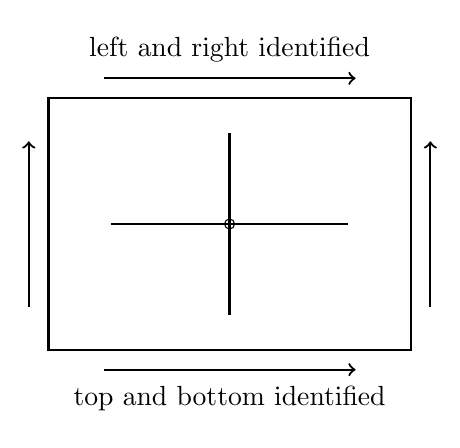
\begin{tikzpicture}[scale=1.0]
\draw[thick] (0,0) rectangle (4.6,3.2);

\draw[->,thick] (0.7,3.45)--(3.9,3.45);
\draw[->,thick] (0.7,-0.25)--(3.9,-0.25);

\draw[->,thick] (-0.25,0.55)--(-0.25,2.65);
\draw[->,thick] (4.85,0.55)--(4.85,2.65);

\draw[thick] (0.8,1.6)--(3.8,1.6);
\draw[thick] (2.3,0.45)--(2.3,2.75);

\draw (2.3,1.6) circle (1.8pt);

\draw (2.3,-0.62) node {top and bottom identified};
\draw (2.3,3.82) node {left and right identified};
\end{tikzpicture}
\caption{通过将矩形的对边等同而构造的平坦环面。这些边不是边界；成对的点是商空间中的同一点。}
\label{fig:c03-flat-torus}
\end{figure}

\begin{classroomqa}
\audiencequestion{那么宇宙能否既平坦又有限？}
\lecturerresponse{可以。平坦性是关于度规的局部陈述；有限性可以是关于拓扑的全局陈述。一个足够大的三维环面在我们能够观测到的整个区域内都会看起来是欧几里得的，尽管其总体积是有限的。\lecturetimestamp{01:13:37--01:17:59}}
\end{classroomqa}

万有覆叠的图像使可观测的后果变得一目了然。不是将边缘等同，而是用基本矩形的副本铺满一个无限欧几里得平面。环面中的一个单一物体在每个副本中都出现一次。在三维中，这些副本形成一个周期性的类晶体阵列。

\begin{classroomqa}
\audiencequestion{我们能否生活在一个环面宇宙中而毫无察觉？}
\lecturerresponse{可以，如果基本胞元大于光已经到达我们的区域。如果它足够小，光就可以穿越这些等同关系，我们就会在不同方向上看到同一批星系的重复图像，甚至可能看到我们自己所在区域的重复景象。无论哪种情况，局部几何都保持平坦。\lecturetimestamp{01:18:16--01:22:04}}
\end{classroomqa}

\begin{classroomqa}
\audiencequestion{为什么球面在其对跖点处停止，而环面却重复？}
\lecturerresponse{在球面上，周围的壳层在\(r=\pi\)处真正收缩到零；所有径向方向都在对跖点处汇聚。在环面上，所选矩形胞元的边缘从不收缩。它与一个同样大的对边等同，因此穿过它会在周期坐标描述中延续同一个空间。\lecturetimestamp{01:22:06--01:23:02}}
\end{classroomqa}

\section{从空间到时空}

我们现在可以恢复时间。在以光速\(c=1\)为单位的单位制中，闵可夫斯基度规为
\begin{equation}
ds^2 = -dt^2 + dx^2 + dy^2 + dz^2.
\label{eq:c03-minkowski}
\end{equation}
符号约定是一种选择；重要的是时间项的符号与空间项的符号相反。光线沿零轨迹传播，
\begin{equation}
ds^2 = 0.
\end{equation}
对于仅沿\(x\)方向的运动，
\begin{equation}
-dt^2 + dx^2 = 0
\qquad\Rightarrow\qquad
dx = \pm dt.
\label{eq:c03-null-flat}
\end{equation}
这两个符号描述光以单位速率向左或向右运动。

对于宇宙学，保留固有时项\(-dt^2\)，将欧几里得空间部分替换为齐性空间度规，并让其整体尺度随时间变化。我们将这个尺度因子记为\(a(t)\)。它现在是一个动力学函数，而不是静态比较中所用的固定半径\(R_c\)。

作为一个可想象的\(2+1\)维例子，取
\begin{equation}
ds^2 = -dt^2 + a(t)^2 d\Omega_2^2.
\label{eq:c03-two-plus-one}
\end{equation}
在每个固定的\(t\)处，空间是一个半径为\(a(t)\)的\(2\)维球面。将这些球面在时间上堆叠起来就给出了时空。熟悉的\(3+1\)维构造是
\begin{equation}
ds^2 = -dt^2 + a(t)^2 d\Sigma^2,
\label{eq:c03-frw-general}
\end{equation}
其中\(d\Sigma^2\)是与时间无关的单位空间度规。三个单连通情形是
\begin{align}
\text{flat:}\quad
ds^2&=-dt^2+a(t)^2\left(dx^2+dy^2+dz^2\right),\label{eq:c03-frw-flat}\\
\text{spherical:}\quad
ds^2&=-dt^2+a(t)^2d\Omega_3^2,\label{eq:c03-frw-spherical}\\
\text{hyperbolic:}\quad
ds^2&=-dt^2+a(t)^2dh_3^2.\label{eq:c03-frw-hyperbolic}
\end{align}
共动坐标的相对尺度是固定的，而\(a(t)\)在变化。在球面和双曲归一化中，\(a(t)\)同时也是瞬时曲率半径。在平坦情形中，其绝对归一化可以吸收进共动坐标。

哈勃定律在任何引力场方程被施加之前就已经成立。考虑两个邻近的共动点，其坐标间隔\(\chi\)固定。它们的物理间隔是
\begin{equation}
D(t)=a(t)\chi.
\label{eq:c03-comoving-distance}
\end{equation}
在固定\(\chi\)下求导给出
\begin{equation}
V=\dot D=\dot a(t)\chi.
\end{equation}
消去\(\chi\)，
\begin{equation}
V = \frac{\dot a}{a} D.
\label{eq:c03-hubble-law}
\end{equation}
因此
\begin{equation}
H = \frac{\dot a}{a}.
\label{eq:c03-hubble-parameter}
\end{equation}
这是均匀膨胀或收缩的运动学恒等式。它对所有三种空间几何都成立：\(\dot a>0\)给出退行，而\(\dot a<0\)给出接近。

仅凭几何并不能确定\(a(t)\)。诸如
\begin{equation}
a(t)\propto t^{2/3},
\qquad
a(t)\propto t^{1/2},
\qquad
a(t)\propto e^{Ht}
\end{equation}
这样的函数都符合均匀度规拟设，但描述的是不同的宇宙物质和能量含量。广义相对论提供了在它们之间进行选择的动力学方程。由此得到的弗里德曼方程还将把平坦、球面和双曲情形与前面发展的牛顿宇宙学中的零能、负能和正能替代情形联系起来。

\begin{classroomqa}
\audiencequestion{几何和宇宙演化会不会比这些模型复杂得多？}
\lecturerresponse{当然会。均匀性和各向同性是限制性假设，之所以被选择，是因为它们自然、在大尺度上观测上成功，并且在数学上易于处理。存在许多更复杂的几何和演化。一个重要的动力学问题是，是否广泛类别的初始不规则模型会演化到这些简单均匀形式之一。\lecturetimestamp{01:36:00--01:36:50}}
\end{classroomqa}

\begin{classroomqa}
\audiencequestion{\(3\)维球面是四维物体的边界吗？}
\lecturerresponse{它可以作为一种嵌入被那样表示，但宇宙学空间就是\(3\)维球面本身。它具有三个内禀维度且没有边界。四维欧几里得图像是可选的脚手架；方程~\eqref{eq:c03-three-sphere}已经完全定义了该几何。\lecturetimestamp{01:36:55--01:37:59}}
\end{classroomqa}

\begin{classroomqa}
\audiencequestion{光度是获得曲率检验所需距离的唯一途径吗？}
\lecturerresponse{不是。谱线识别红移，邻近距离阶梯校准哈勃关系，而超新星提供近似标准的光度。这些方法被相互交叉检验，而不是孤立地信任。甚至平方反比光度定律也依赖于几何，因为光波前的面积由\(r^2\)、\(\sin^2r\)或\(\sinh^2r\)决定。若干观测量的一致性才是支持近平坦性的依据。\lecturetimestamp{01:38:00--01:41:07}}
\end{classroomqa}

\section{需要继续推进的内容}

均匀宇宙的几何可以从围绕任意观测者的球壳的增长中读出：
\begin{equation}
f(r)=
\begin{cases}
r, & \text{flat space},\\
\sin r, & \text{positive curvature},\\
\sinh r, & \text{negative curvature}.
\end{cases}
\end{equation}
空间度规是\(dr^2+f(r)^2d\Omega_{n-1}^2\)。同一个函数控制角大小以及球壳上可用的天体数目，因此曲率具有直接的观测意义。大的曲率半径在局部隐藏了这些差异，而环面式的认同表明局部曲率本身并不决定整体大小或拓扑。

加入\(-dt^2\)和公共因子\(a(t)^2\)，就把三种均匀空间度规中的任何一种变成了宇宙学时空。它立即给出\(V=HD\)，其中\(H=\dot a/a\)，但它使\(a(t)\)未被确定。因此下一步不再是另一个几何练习。它是动力学问题：利用爱因斯坦方程来确定物质、辐射、曲率以及其他形式的能量如何使尺度因子演化。
